\documentclass{article}
\usepackage[utf8]{inputenc}
\usepackage[a4paper, total={6in, 9in}]{geometry}
\usepackage[francais]{babel}
\usepackage{natbib}
\usepackage{graphicx, caption, float}
\usepackage{listings, lstautogobble}

\setlength{\parindent}{0pt}
\newcommand{\HRule}{\rule{\linewidth}{0.5mm}}

\begin{document}


\begin{titlepage}
\begin{center}


\textsc{\LARGE \'Ecole Polytechnique Fédérale de Lausanne}


\includegraphics[width=0.3\textwidth]{EPFL_logo.jpg}~\\[5cm]
% Title

{ \huge \bfseries Databases Project \\[0.4cm] }

\HRule \\[0.4cm]

{ \huge \emph{First and Second deliverable} \\[6cm] }

% Author and supervisor
\noindent
\begin{minipage}{0.4\textwidth}
\begin{center} \large
\emph{Authors:}\\
Valentine \textsc{Arrieta}\\
Morgan \textsc{Bruhin}\\
Tristan \textsc{Overney}

\end{center}
\end{minipage}%


\vfill

% Bottom of the page
{\large \today}

\end{center}
\end{titlepage}

\section{First deliverable}
\subsection{ER model}

    \begin{figure}[H]
        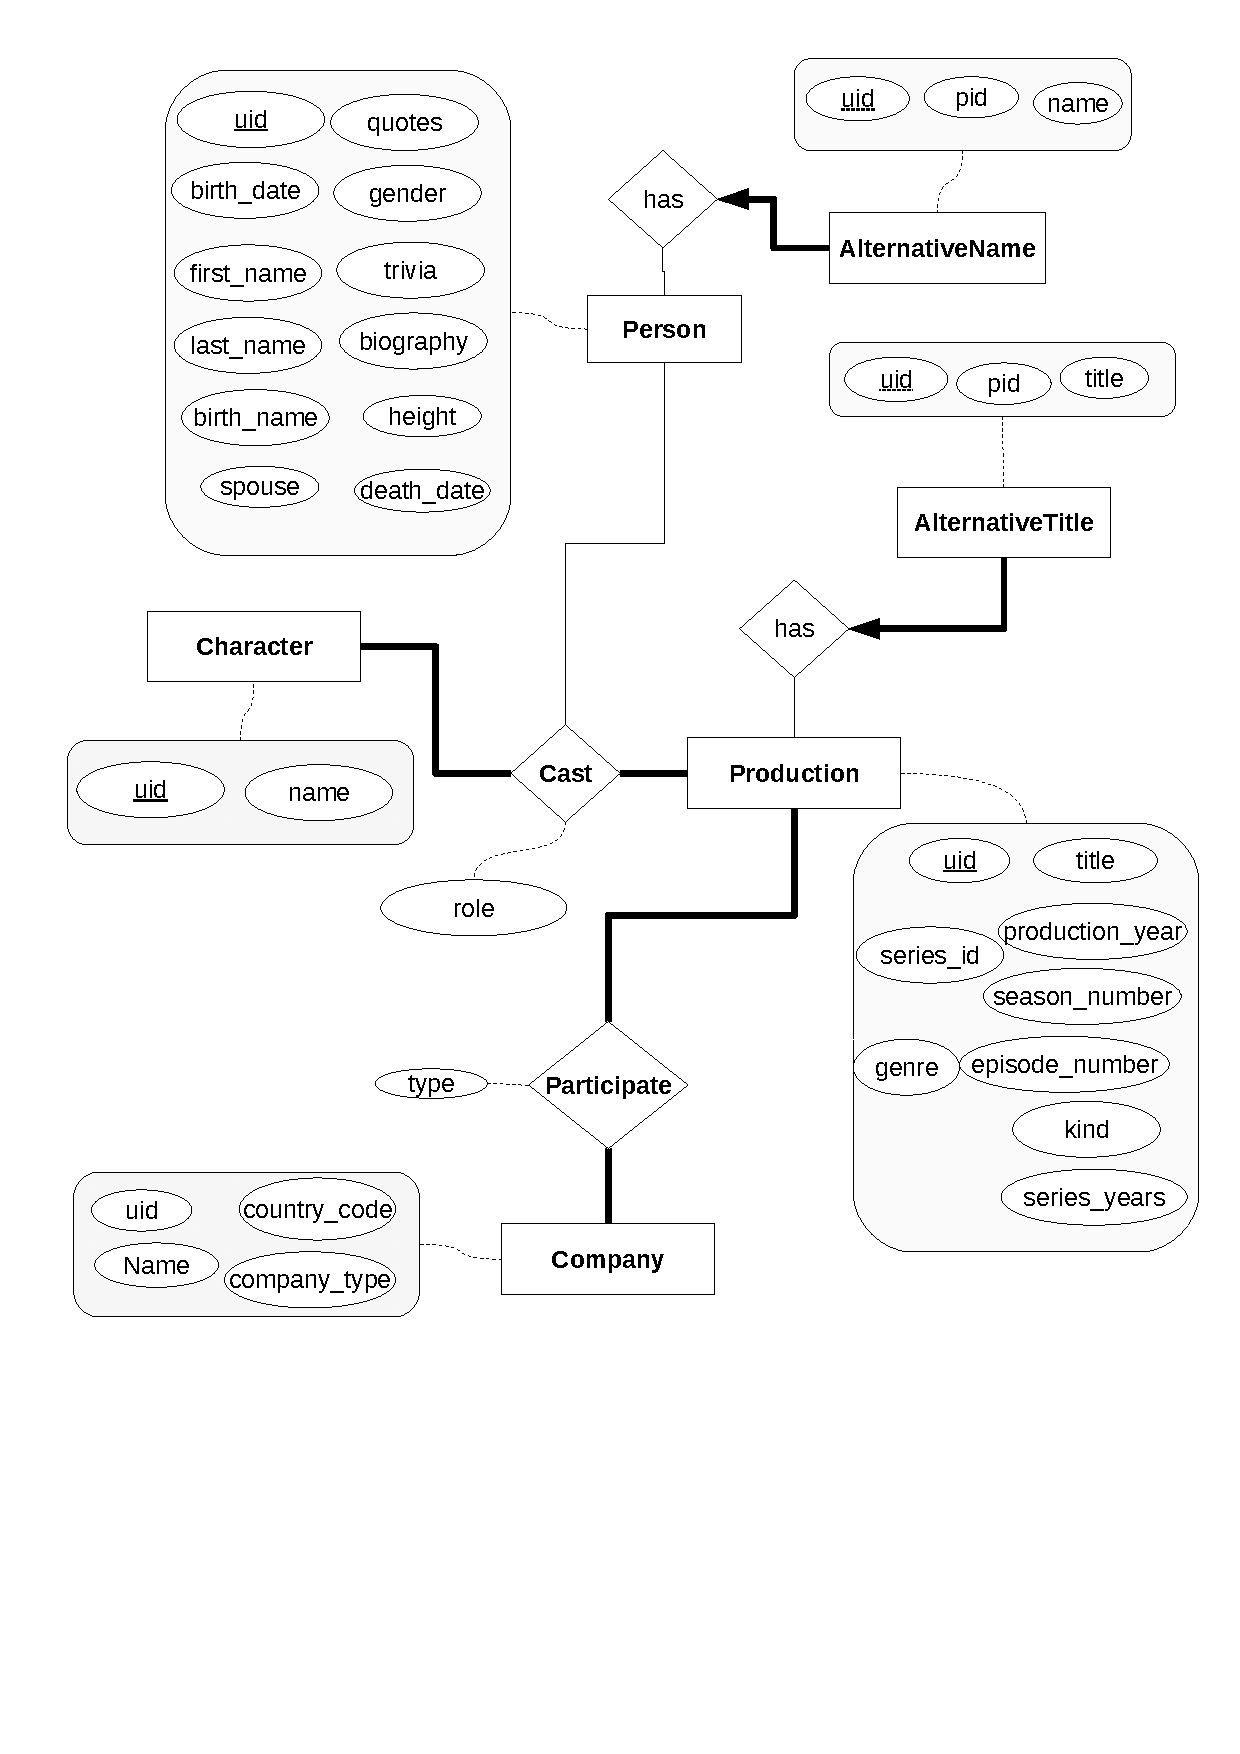
\includegraphics[width=\linewidth]{Diagrame_ER.pdf}
        \captionsetup{justification=centering}
        \caption{ER model of our DBMS}
    \end{figure}

\subsection{Table creation}
    We will implement the next deliverables using our own server with PostGreSQL.
    As such the types used in the following CREATE TABLE possibly doesn't work well in an
    Oracle DB environnement.
    \begin{lstlisting}[
           language=SQL,
           showspaces=false,
           basicstyle=\ttfamily,
           autogobble=true,
           commentstyle=\color{gray}
        ]
    CREATE TABLE person
       (uid INTEGER NOT NULL,
        first_name CHAR(75) NOT NULL,
        last_name CHAR(75) NOT NULL,
        gender CHAR(1),
        trivia TEXT,
        quotes VARCHAR(4000),
        birth DATE,
        death DATE,
        biography TEXT,
        spouse CHAR(100),
        height DOUBLE PRECISION,
        primary key (uid));

    CREATE TABLE alternative_name
       (uid INTEGER NOT NULL,
        pid INTEGER NOT NULL,
        name CHAR(60) NOT NULL,
        primary key (uid),
        foreign key (pid) references person(uid)
        ON DELETE CASCADE);
    
    CREATE TABLE character
       (uid INTEGER NOT NULL,
        name CHAR(60) NOT NULL,
        primary key (uid));
    
    CREATE TYPE CAST_ROLE AS
        ENUM ('actor', 'actress', 'producer', 'writer', 'cinematographer',
        'composer', 'costume designer', 'director', 'editor', 'miscellaneous crew',
        'production designer');
    
    CREATE TABLE production
       (uid INTEGER NOT NULL,
        title CHAR(80) NOT NULL,
        production_year DATE,
        genre CHAR(20),
        primary key (uid));
    
    CREATE TABLE casting
       (cid INTEGER,
        perid INTEGER NOT NULL,
        prodid INTEGER NOT NULL,
        role CAST_ROLE NOT NULL,
        primary key (cid, perid, prodid, role),
        foreign key (cid) references character (uid),
        foreign key (perid) references person (uid),
        foreign key (prodid) references production (uid));
    
    
    CREATE TABLE tv_serie
       (series_years CHAR(11),
        primary key (uid)) INHERITS (Production);
    
    CREATE TABLE episode
       (sid INTEGER NOT NULL,
        season SMALLINT NOT NULL,
        episode SMALLINT NOT NULL,
        primary key (uid),
        foreign key (sid) references tv_serie (uid)
        ON DELETE CASCADE) INHERITS (production);
    
    CREATE TABLE tv_movie
        (primary key (uid)) INHERITS (production);
    
    CREATE TABLE movie
        (primary key (uid)) INHERITS (production);
    
    CREATE TABLE video_movie
        (primary key (uid)) INHERITS (production);
    
    CREATE TABLE video_game
        (primary key (uid)) INHERITS (production);
    
    CREATE TYPE COMPANY_TYPE AS ENUM ('distributors', 'production company');
    
    CREATE TABLE company
       (uid INTEGER NOT NULL,
        name CHAR(80) NOT NULL,
        country_code CHAR(6),
        primary key (uid));
    
    CREATE TABLE participate
       (pid INTEGER NOT NULL,
        cid INTEGER NOT NULL,
        type COMPANY_TYPE NOT NULL,
        primary key (pid, cid),
        foreign key (pid) references production(uid),
        foreign key (cid) references company(uid));
    
    CREATE TABLE alternative_title
       (uid INTEGER NOT NULL,
        pid INTEGER NOT NULL,
        title CHAR (80) NOT NULL,
        primary key (uid),
        foreign key (pid) references production (uid)
        ON DELETE CASCADE);
    \end{lstlisting}

\pagebreak
\subsection{Discussion about constraint}
    A person can have one or more alternative name but an alternative name can describe only one person. We thus have a one-to-many relationship set. Also if the person is deleted from the database, his alternative names (if any) will be too. We thus created a weak entity for alternative name.
    We applied the same design choice for two similar situations: the production and its alternative title(s) and the tv serie and its episode(s). \\
    
    A production cast make the connection between the production, the person and the character (if any). We thus made a ternary relationship between the three entity person, character and production. We add the role of the person as an attribute of the relationship set. A character exist only if related to at least one person and one production. The person and production entity don't have this constraint since a production can have only a director that won't have any character.  \\
    
    Companies can be involved into production. They can play roles of different type (for example production, distribution), thus we added an attribute to the relationship "participate" called type instead of having a lot of duplicated entries in the "Company" table. Since that design choice, the data set given has been changed and comforted us in our design choice as the "type" attribute has been moved out of the COMPANY.csv file. A production need to have at least one company involved.\\
    
    We used enums for both the company type and the cast role because their value options are limited. As such we'll avoid repeating a considerable amount of bytes between the many lines sharing the same value for that field.\\
    
    And last but not least, instead of having a huge melting pot table called production, we made a "parent table" with all the fields shared between the different kinds of production and then we have a table per production kind which inherit from the production table and where some kind have additional info such as the season number in episode. This is the implementation of an IS A relationship in PostGreSQL. This allow us again to avoid having many entries of a table with some null field that they'd never have a value for.

\pagebreak
\section{Second deliverable}

\subsection{First deliverable changes}


\subsection{SQL queries}

A) Number of movies per production year
    \begin{lstlisting}[
           language=SQL,
           showspaces=false,
           basicstyle=\ttfamily,
           autogobble=true,
           commentstyle=\color{gray}
        ]
        
    SELECT production_year, COUNT(*) FROM production
    WHERE (kind = 'movie'
        OR kind = 'tv movie'
        OR kind = 'video movie')
        AND production_year IS NOT NULL
    GROUP BY production_year
    ORDER BY production_year ASC;
    \end{lstlisting}
\medskip

B) Top 10 countries with the most production companies
    \begin{lstlisting}[
           language=SQL,
           showspaces=false,
           basicstyle=\ttfamily,
           autogobble=true,
           commentstyle=\color{gray}
        ]

    SELECT c.country_code, COUNT(DISTINCT c.uid) AS count 
    FROM company c
    LEFT JOIN participate par ON c.uid = par.cid
    WHERE par.type = 'production companies'
        AND c.country_code IS NOT NULL
    GROUP BY c.country_code
    ORDER BY count DESC LIMIT 10;
    \end{lstlisting}
    
\medskip

C) Compute the min, max and average career duration
    \begin{lstlisting}[
           language=SQL,
           showspaces=false,
           basicstyle=\ttfamily,
           autogobble=true,
           commentstyle=\color{gray}
        ]
        
    SELECT avg(duration) AS avg_duration, MAX(duration) AS max_duration, 
    MIN(duration) AS min_duration
    FROM (  
        SELECT (1+(MAX(prod.production_year)-MIN(prod.production_year))) 
        AS duration
        FROM casting c, production prod
        WHERE c.prodid = prod.uid
        GROUP BY c.perid
        ) AS career_duration;
    \end{lstlisting}
\medskip

D) Compute the min, max and average number of actors in a production
    \begin{lstlisting}[
           language=SQL,
           showspaces=false,
           basicstyle=\ttfamily,
           autogobble=true,
           commentstyle=\color{gray}
        ]
        
    SELECT avg(numb) AS avg_nb_act, MAX(numb) AS max_nb_act, 
    MIN(numb) AS min_nb_act
    FROM (  SELECT count(*) AS numb
            FROM casting
            WHERE role = 'actor'
            GROUP BY prodid
    ) AS number;
    \end{lstlisting}
\medskip

E) Min, Max, Avg height of female persons
    \begin{lstlisting}[
           language=SQL,
           showspaces=false,
           basicstyle=\ttfamily,
           autogobble=true,
           commentstyle=\color{gray}
        ]
        
    SELECT MIN(height) AS min_height, MAX(height) AS max_height, 
    AVG(height) AS avg_height 
    FROM person
    WHERE gender = 'f';
    \end{lstlisting}
\medskip

F) List all pairs of persons and movies where the person has both directed the movie and acted in the movie. Do not include tv and videos movies
    \begin{lstlisting}[
           language=SQL,
           showspaces=false,
           basicstyle=\ttfamily,
           autogobble=true,
           commentstyle=\color{gray}
        ]
        
    SELECT p2.uid, p1.uid, person.first_name, person.last_name, 
    prod.title, p1.role, p2.role 
    FROM casting p1
    LEFT JOIN casting p2 ON p1.prodid = p2.prodid AND p1.perid = p2.perid
    LEFT JOIN person ON p1.perid = person.uid
    LEFT JOIN production prod ON p1.prodid = prod.uid
    WHERE p1.role='director' AND p2.role='actor';
    \end{lstlisting}
\medskip

G) List the three most popular character names
    \begin{lstlisting}[
           language=SQL,
           showspaces=false,
           basicstyle=\ttfamily,
           autogobble=true,
           commentstyle=\color{gray}
        ]
        
    SELECT name, COUNT(*) AS amount
    FROM character
    GROUP BY name
    ORDER BY amount DESC LIMIT 3;
    \end{lstlisting}
\medskip

\subsection{Interface}

\end{document}
